%%%%
%       _  _____  ___  _____  _   _  ___ 
%      / \|_   _||_ _||_   _|| | | |/ __|
%     / △ \ | |   | |   | |  | |_| |\__ \
%    /_/¯\_\|_|  |___|  |_|   \___/ |___/
%                 EDUCAÇÃO
%    Modelo de TCC - Ciência da Computação
%%%%

\documentclass[12pt]{article}

\usepackage{sbc-template}
\usepackage{graphicx, url}
\usepackage[utf8x]{inputenc}
\usepackage[brazil]{babel}
\usepackage[T1]{fontenc}
\usepackage[english=american]{csquotes}
\usepackage{float}
\usepackage{comment}
\usepackage{amsmath}
\usepackage{amssymb}
\usepackage{enumerate}
\usepackage{subcaption}
\usepackage{setspace}
\usepackage{listings}
\usepackage{inconsolata}
\usepackage{tabularray}
%\usepackage[backref=page]{hyperref}
%\hypersetup{
%    colorlinks=true,
%    allcolors=blue,
%}

% %%%%%%%%%%%%%%%%%%%%%%%%%%%%%%%%%%%%%%%%%%%%%%%%%%%%%%%%%%%%%%
% define o modelo de referencias
\usepackage[style=abnt]{biblatex}

% indica o arquivo com as referencis bibliograficas
\addbibresource{sbc-template.bib}

% carrega o pacote com alterações para Computação Atitus
\usepackage{sty/cc_atitus}
% %%%%%%%%%%%%%%%%%%%%%%%%%%%%%%%%%%%%%%%%%%%%%%%%%%%%%%%%%%%%%%

% %%%%%%%%%%%%%%%%%%%%%%%%%%%%%%%%%%%%%%%%%%%%%%%%%%%%%%%%%%%%%%
% REFERENCIAS DEVERÃO SER INCLUÍDAS NO ARQUIVO: sbc-template.bib
%
% SOBRE CITAÇÕES:
% Para citar no padrão '(Autores, ano)' use: \cite{chave}
% Para citar no padrão 'Autores (ano)'  use: \textcite{chave} ou \citeonline{chave}
% Para citar no padrão 'Autores'        use: \citelastname{chave}
% Para citar no padrão '(Autor, 2009c; Outro Autor, 2009; Outro Autor, 2015)' use: \cites{chave1}{chave2}{chave3}
% Para citar no padrão 'Autor (ano), Autor (ano) e Autor (ano)' use: \textcites{chave1}{chave2}{chave3}

% Demais exemplos ver documento:
%  https://github.com/abntex/biblatex-abnt/raw/master/doc/biblatex-abnt.pdf
%
% Normas ABNT: https://usp.br/sddarquivos/arquivos/citacoes10520.pdf
%              https://usp.br/sddarquivos/arquivos/abnt6023.pdf
%
% %%%%%%%%%%%%%%%%%%%%%%%%%%%%%%%%%%%%%%%%%%%%%%%%%%%%%%%%%%%%%%
% Atualizações no modelo
% 2024-09-23: (fahadkalil) Ajuste para quebra automática de linhas nas células de uma tabela
% 2024-10-17: (fahadkalil) Inserção de comentários com outras citações e indicação de uso do comando "\enquote"
% %%%%%%%%%%%%%%%%%%%%%%%%%%%%%%%%%%%%%%%%%%%%%%%%%%%%%%%%%%%%%%
% CABEÇALHO
\title{Extração de Backbone para Reduzir o Tempo de Solução do Problema de Maximização de Influência em Redes Sociais}

\author{Ana Luiza Almeida Soares\inst{1}, Rodrigo César Pedrosa Silva\inst{1}} % autor principal, orientador

\address{Programa de Pós-Graduação em Ciência da Computação \\ Departamento de Computação \\ Universidade Federal de Ouro Preto
\email{ana.almeida3@aluno.ufop.edu.br, rodrigo.silva@ufop.edu.br}
}
% %%%%%%%%%%%%%%%%%%%%%%%%%%%%%%%%%%%%%%%%%%%%%%%%%%%%%%%%%%%%%%

\begin{document}
\maketitle % Não remova essa linha!

% \begin{abstract} % resumo em inglês
%   Escreva seu resumo em língua estrangeira (inglês)...
% \end{abstract}
     
% \begin{resumo}
%   Resumo do trabalho (português)...  
% \end{resumo}

\section{Introdução}

As redes sociais têm se mostrado ferramentas poderosas para resolver uma ampla gama de problemas em diferentes áreas. Essas redes não se restringem apenas a plataformas digitais como Facebook, Twitter e Instagram, mas também são aplicáveis em contextos que envolvem interações entre elementos, como a disseminação de informações, a propagação de doenças, e a maximização de influência em campanhas de marketing. Sendo assim, em contextos como o espalhamento de notícias ou epidemias, a compreensão da estrutura da rede é crucial para prever e controlar o fluxo de informações ou patógenos.

O problema de Maximização de Influência busca identificar o conjunto de pessoas que maximiza a propagação de influência em uma rede social. Em outras palavras, considerando uma rede social onde os nós representam pessoas e as arestas indicam o nível de influência que uma pessoa exerce sobre outra, o objetivo é encontrar o conjunto de nós que maximize o número de outros nós influenciados.

Esse problema possui inúmeras aplicações, desde a divulgação de produtos em redes sociais até a análise da eficácia da disseminação de informações políticas. O campo vem sendo amplamente estudado devido ao impacto significativo que as redes sociais digitais exercem na formação da opinião pública.

A solução ideal para o problema envolveria avaliar todas as permutações possíveis de conjuntos, mas isso é inviável para redes grandes, devido ao tempo necessário para construir e comparar cada permutação em busca da melhor. 

Consequentemente, várias abordagens foram desenvolvidas. Uma das abordagens utilizadas para lidar com a complexidade do problema de Maximização de Influência é reduzir o tamanho da rede, simplificando o problema e, teoricamente, diminuindo o tempo necessário para encontrar uma solução. Uma técnica comum para isso é a utilização do "backbone" da rede, que consiste em identificar e manter apenas os nós e arestas mais importantes para a propagação de influência, enquanto remove elementos menos relevantes.

A ideia central dessa abordagem é que, ao resolver o problema de maximização de influência em uma rede reduzida, ou backbone, o tempo de processamento é significativamente menor, sem perda substancial de precisão. A hipótese é que, uma vez obtido o conjunto de nós influentes no backbone, o espalhamento da influência na rede original pode ser estimado de maneira eficaz, com uma quantidade de nós influenciados semelhante àquela que seria obtida em uma análise completa da rede.

Essa estratégia oferece uma solução mais eficiente, mantendo o desempenho aproximado das abordagens tradicionais, mas com uma redução substancial no custo computacional.

\subsection{Objetivos}

O objetivo deste estudo é investigar a aplicação da técnica de extração de backbone na estrutura de redes sociais e avaliar seus efeitos no desempenho computacional e na qualidade dos resultados do problema de maximização de influência. Especificamente, buscamos:
\begin{itemize}
    \item Investigar o impacto da extração de backbone na estrutura de redes sociais: Analisar como a redução da rede para um backbone afeta a propagação de influência e a representação da rede original, identificando os nós e arestas essenciais para a dinâmica de disseminação.
    \item Avaliar a influência do backbone na eficiência computacional do problema de maximização de influência: Examinar o impacto da utilização de backbone na redução do tempo de processamento necessário para resolver o problema de maximização de influência, comparando a abordagem com o modelo completo da rede.
    \item Identificar possíveis ganhos ou perdas em termos de tempo de execução e qualidade dos resultados: Verificar se a abordagem de backbone resulta em ganhos significativos de tempo sem comprometer a precisão da estimativa do número de nós influenciados, ou se há perdas notáveis na qualidade dos resultados em termos de alcance da influência. 
\end{itemize}

% \section{Referencial Teórico}
% Voltado ao objetivo geral (teoria por trás do método), deve conter os assuntos bases da pesquisa, fazendo citações indiretas e diretas curtas.

% \begin{comment}
% testando comentario
% \end{comment}

% \begin{description}
%     \item[Exemplos de citação indireta]    
% \end{description}

% Segundo \textcite{spinello2024}, o trabalho de conclusão deve ter citações retiradas de artigos científicos encontrados nas bases de dados. 

% O trabalho de conclusão deve ter citações retiradas de artigos científicos encontrados nas bases de dados \cite{spinello2024}.

% \begin{description}
%     \item[Exemplos de citação direta curta]
% \end{description}

% Segundo \textcite{spinello2024} \enquote{o trabalho de conclusão deve ter citações retiradas de artigos científicos encontrados nas bases de dados}. Note que para colocar um texto entre aspas, usamos o comando \verb|\enquote{texto}|.

% Ressalta-se que o \enquote{trabalho de conclusão deve ter citações retiradas de artigos científicos encontrados nas bases de dados} \cite{spinello2024}.

% No estudo comparativo apresentado em \textcite[p. 107]{rabello2010} ...

% No trabalho de \textcite{pargaonkar2021} ...

% Nos trabalhos de \textcites{badgujar2024}{pargaonkar2021} são aplicadas técnicas de ...

% No artigo de \textcite{estevao2023} ...

% \textsc{Citação direta longa devem ser evitadas em artigos científicos!}

% \section{Trabalhos Relacionados}

% Trabalhos semelhantes aos objetivos específicos, sempre detalhando ao final da seção a
% diferença ao trabalho proposto (quantidade -- 5 trabalhos);

% Neste item serão apresentados os principais trabalhos que possuem uma relação com o assunto definido neste estudo....

% % Itens com marcadores
% \begin{itemize}
%      \item \textbf{Título do artigo 01 \cite{ogliari2019}}
     
%      Primeiro parágrafo indicar uma introdução do assunto... \\
%      No segundo: o que o estudo procurou analisar, qual o objetivo... \\
%      No terceiro: o que foi desenvolvido, qual aplicação/experimento foi realizado... \\
%      Último: em quais conclusões o trabalho chegou... \\
         
%     \item \textbf{Título do artigo 02 (Autor, ano)}
    
%      Primeiro parágrafo indicar uma introdução do assunto... \\
%      No segundo: o que o estudo procurou analisar, qual o objetivo... \\
%      No terceiro: o que foi desenvolvido, qual aplicação/experimento foi realizado... \\
%      Último: em quais conclusões o trabalho chegou... \\
    
%     \item \ldots
% \end{itemize}

\section{Materiais e Métodos}

A metodologia adotada para este trabalho envolve a análise de redes sociais a partir da extração do backbone, seguida da aplicação de um algoritmo de maximização de influência. O processo será realizado em duas etapas: uma para a rede completa e outra para o backbone extraído.

Primeiramente, serão selecionadas três redes sociais como estudo de caso. A partir dessas redes, será extraído o backbone, que consiste em uma versão simplificada da rede, mantendo apenas os nós e arestas mais relevantes para a propagação de influência. Em seguida, será aplicado um algoritmo de maximização de influência para identificar o conjunto de nós influentes em ambas as versões da rede, tanto na rede completa quanto no backbone.

Com os nós influentes identificados, será calculado o espalhamento, ou seja, a quantidade de nós influenciados em cada rede. O tempo de execução do algoritmo será registrado para ambas as redes, e os resultados serão comparados para avaliar as diferenças em termos de número de nós influenciados e eficiência computacional. O objetivo é verificar se a utilização do backbone resulta em uma redução significativa no tempo de processamento, mantendo uma qualidade similar na quantidade de nós influenciados em relação à rede completa.  

As redes sociais escolhidas para a experimentação foram obtidas a partir dos sites disponibilizados pelo Professor Dr. Vander Freitas na disciplina \textit{PCC 121 Redes Complexas}. Essas redes representam páginas do Facebook (verificadas, ou seja, páginas azuis) de diferentes categorias, e os nós representam as páginas enquanto as arestas representam as "curtidas mútuas" entre elas. Porém, devido a limitações de tempo, só foi possível executar para a rede 1. Abaixo estão as redes selecionadas para o estudo:

\begin{enumerate}
    \item \textbf{Site:} \url{https://networkrepository.com/fb-pages-politician.php} \\
    \textbf{Nós:} 5.900 \\
    \textbf{Arestas:} 41.700
    
    \item \textbf{Site:} \url{https://networkrepository.com/fb-pages-food.php} \\
    \textbf{Nós:} 620 \\
    \textbf{Arestas:} 2.100
    
    \item \textbf{Site:} \url{https://networkrepository.com/fb-pages-artist.php} \\
    \textbf{Nós:} 50.500 \\
    \textbf{Arestas:} 819.100
\end{enumerate}

    % Tecnologias, instrumentos e procedimentos que serão usados no estudo. O Algoritmo \ref{alg:id_algo} se refere ao método de ordenação Bubblesort expresso em linguagem Python.

    % % Código-fonte formatado
    % % Ver: https://en.wikibooks.org/wiki/LaTeX/Source_Code_Listings
    % \begin{lstlisting}[  
    %     %float,
    %     language=Python, 
    %     frame=single, 
    %     numbers=left,
    %     caption={Método de ordenação Bubblesort},
    %     label={alg:id_algo} % id para referenciar
    %     ]        
    % def bubble_sort(alist):
    %     for i in range(len(alist)-1,0,-1):
    %         for j in range(i):
    %             if alist[i]>alist[i+1]:
    %                 temp = alist[i]
    %                 alist[i] = alist[i+1]
    %                 alist[i+1] = temp    
    % \end{lstlisting}

    % % Figura
    % % https://pt.overleaf.com/learn/latex/Inserting_Images
    % \begin{figure}[H]
    %     \centering
    %     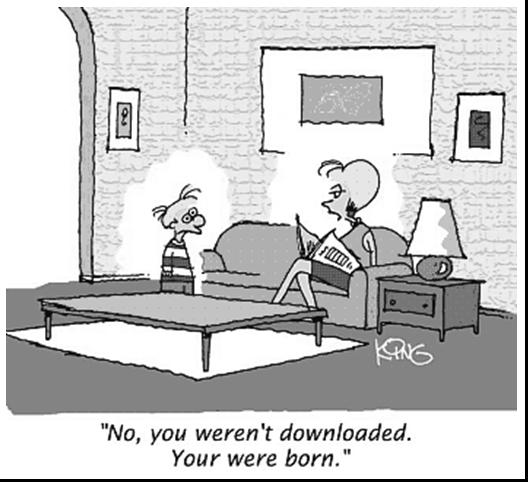
\includegraphics[width=0.5\textwidth]{fig1.jpg}
    %     \caption{Minha figura}
    %     \label{fig:id_figura}
    % \end{figure}
    
    % % Tabela
    % % Editor online: https://www.latex-tables.com
    %  \begin{table}[ht]
    %     \centering
    %     \caption{Minha tabela}
    %     \label{tab:id_tabela}
    %     \begin{tblr}{
    %       colspec = {X[l] X[l]}, % Tipo X define células com quebra automática de linha. Use: l=left, r=right, c=center ou j=justify para alinhamento dentro das células
    %       width = \linewidth,
    %       hlines, % inclui borda horizontal
    %       vlines, % inclui borda vertical        
    %     }
    %     \textbf{cabeçalho 1} & \textbf{cabeçalho 2} \\
    %     {texto à esquerda} & {Existem muitas variações das passagens do Lorem Ipsum disponíveis, mas a maior parte sofreu alterações de alguma forma, pela injecção de humor, ou de palavras aleatórias que nem sequer parecem suficientemente credíveis. Se vai usar uma passagem do Lorem Ipsum, deve ter a certeza que não contém nada de embaraçoso escondido no meio do texto.}
    %     \end{tblr}
    % \end{table}

\section{Resultados Obtidos}

A tabela a seguir apresenta os resultados obtidos para o problema de maximização de influência, tanto para a rede completa quanto para a rede com backbone extraído.

\begin{table}[ht]
\centering
\begin{tabular}{|c|c|c|c|}
\hline
\textbf{Configuração} & \textbf{Tempo de Execução} & \textbf{Nós Influenciados} & \textbf{Taxa} \\ \hline
Com Backbone           & 10 min 31 seg              & 456 nós                    & 98,32\%  de acerto               \\ \hline
Sem Backbone           & 13 min 37 seg              & 478 nós                    & 23,15\% de redução                       \\ \hline
\end{tabular}
\caption{Resultados de execução do algoritmo de maximização de influência com e sem Backbone}
\end{table}

Os resultados indicam que o uso do backbone proporcionou uma redução no tempo de execução. Quando o algoritmo foi executado com o backbone, o tempo total foi de 10 minutos e 31 segundos, enquanto na rede completa o tempo foi de 13 minutos e 37 segundos, o que representa uma redução de 23,15\%* no tempo de processamento. Essa melhoria é atribuída à simplificação da rede, que resultou em menor número de nós e arestas, permitindo uma execução mais rápida.

Em termos de quantidade de nós influenciados, a rede com backbone resultou em 456 nós influenciados, enquanto a rede completa influenciou 478 nós. A diferença de 22 nós é pequena, representando uma redução de aproximadamente 4,6\% na quantidade de nós influenciados ao se utilizar o backbone. Esse pequeno desvio está dentro do esperado, já que a rede com backbone é uma versão simplificada, com menos conectividade.

A taxa de acerto, calculada como a proporção de nós influenciados na rede com backbone em relação à rede completa, foi de 98,32\%. Isso significa que, apesar da redução no número de nós influenciados, o algoritmo foi capaz de aproximar a solução da rede completa com uma margem de erro muito pequena. Esse resultado indica que o uso do backbone não compromete substancialmente a qualidade da previsão, mantendo uma alta precisão na identificação dos nós influenciados.

Em resumo, os resultados sugerem que a utilização do backbone trouxe uma significativa redução no tempo de execução (23,15\%) com uma ligeira perda na quantidade de nós influenciados (4,6\%), mas com uma taxa de acerto de 98,32\%, indicando que a abordagem é eficiente em termos de tempo, mantendo uma boa qualidade nos resultados.
    


    

% \section{Considerações Finais}
% Essa seção deverá ser escrita na segunda parte do trabalho, conhecida como TCC2.

% %%%%%%%%%%%%%%%%%%%%%%%%%%%%%%%%%%%%%%%%%%%%%%%%%%%%%%%%%%%%%%
% Seção de Referências (gerada automaticamente)
\printbibliography  % Não remover esta linha
% %%%%%%%%%%%%%%%%%%%%%%%%%%%%%%%%%%%%%%%%%%%%%%%%%%%%%%%%%%%%%%

\end{document}